\documentclass{article}
\usepackage{hyperref}
\usepackage{amsmath,amssymb}
\usepackage{graphicx}


\title{\bf{CSE397: Assignment \#1}}
\author{Nicholas Malaya \\ Institute for Computational Engineering and Sciences \\ University of Texas at Austin} \date{}

\begin{document}
\maketitle

\newpage
\section{Problem 1}

\begin{figure}[p]
  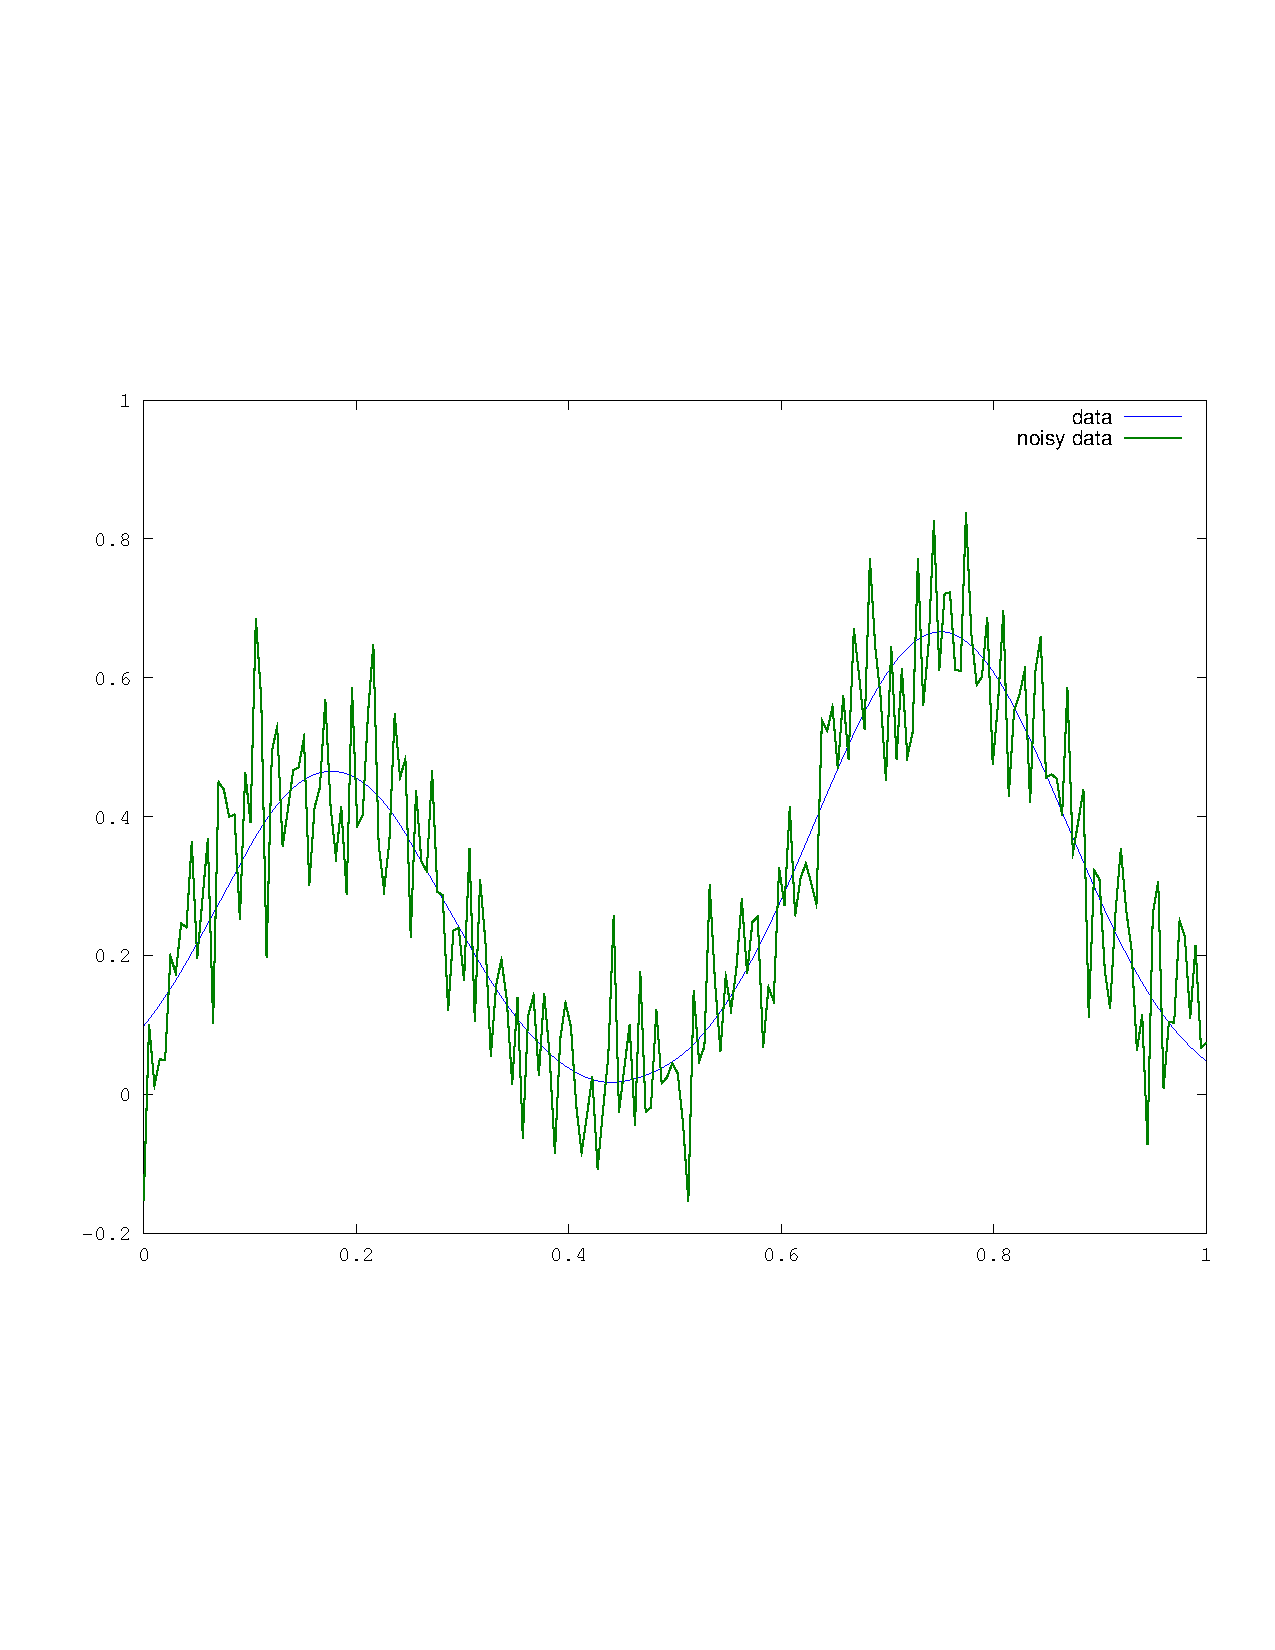
\includegraphics[scale=.5]{plots/data.pdf}
  \label{fig:data}
  \caption{The data (after applying the filter) with and without normally distributed noise. }
\end{figure}

After applying the new filter $k(x)$ and adding gaussian noise, the data used as input for the inverse problem is plotted in figure \ref{fig:data}. 

\end{document}